\documentclass[9pt,twocolumn,twoside,final]{pnas-new}

% Use the lineno option to display guide line numbers if required.
% Note that the use of elements such as single-column equations
% may affect the guide line number alignment.


\usepackage[T1]{fontenc}
\usepackage[utf8]{inputenc}

% tightlist command for lists without linebreak
\providecommand{\tightlist}{%
  \setlength{\itemsep}{0pt}\setlength{\parskip}{0pt}}


% Pandoc citation processing
%From Pandoc 3.1.8
% definitions for citeproc citations
\NewDocumentCommand\citeproctext{}{}
\NewDocumentCommand\citeproc{mm}{%
  \begingroup\def\citeproctext{#2}\cite{#1}\endgroup}
\makeatletter
 % allow citations to break across lines
 \let\@cite@ofmt\@firstofone
 % avoid brackets around text for \cite:
 \def\@biblabel#1{}
 \def\@cite#1#2{{#1\if@tempswa , #2\fi}}
\makeatother
\newlength{\cslhangindent}
\setlength{\cslhangindent}{1.5em}
\newlength{\csllabelwidth}
\setlength{\csllabelwidth}{3em}
\newenvironment{CSLReferences}[2] % #1 hanging-indent, #2 entry-spacing
 {\begin{list}{}{%
  \setlength{\itemindent}{0pt}
  \setlength{\leftmargin}{0pt}
  \setlength{\parsep}{0pt}
  % turn on hanging indent if param 1 is 1
  \ifodd #1
   \setlength{\leftmargin}{\cslhangindent}
   \setlength{\itemindent}{-1\cslhangindent}
  \fi
  % set entry spacing
  \setlength{\itemsep}{#2\baselineskip}}}
 {\end{list}}
\usepackage{calc}
\newcommand{\CSLBlock}[1]{#1\hfill\break}
\newcommand{\CSLLeftMargin}[1]{\parbox[t]{\csllabelwidth}{#1}}
\newcommand{\CSLRightInline}[1]{\parbox[t]{\linewidth - \csllabelwidth}{#1}\break}
\newcommand{\CSLIndent}[1]{\hspace{\cslhangindent}#1}


\templatetype{pnasresearcharticle}  % Choose template

\title{Comment la diversité spécifique du benthos varie-t-elle dans les
rivières du Québec?}

\author[a]{Léanne Beauregard}
\author[a]{Élyse Castilloux}
\author[a]{Maude Roy}
\author[a]{Erick-Daniel Vasquez}

  \affil[a]{Univeristé de Sherbrooke, Département de Biologie}


% Please give the surname of the lead author for the running footer
\leadauthor{Anonymous}

% Please add here a significance statement to explain the relevance of your work
%\significancestatement{}


\authorcontributions{}



\correspondingauthor{\textsuperscript{} }

% Keywords are not mandatory, but authors are strongly encouraged to provide them. If provided, please include two to five keywords, separated by the pipe symbol, e.g:
 \keywords{  Benthos |  Rivière  } 

\begin{abstract}
Dans le cadre du cours de Méthodes en écologie computationnelle (BIO500)
nous avons analysé les données de 43 rivières, récoltées entre 2016 et
2021, sur la biodiversité benthique sur les rivières du Québec. Plus
précisément, nous avons cherché à comprendre comment la diversité
spécifique du benthos varie en fonction de la vitesse du courant, de la
profondeur de la rivière et de la température de l'eau. Contrairement à
ce que nous pensions, les résultats démontrent que seule la température
de l'eau affecte significativement la richesse spécifique du benthos,
mais que ce facteur n'explique qu'une infime partie de sa variance
spatiale.
\end{abstract}

\dates{This manuscript was compiled on \today}
\doi{\url{www.pnas.org/cgi/doi/10.1073/pnas.XXXXXXXXXX}}

\begin{document}

% Optional adjustment to line up main text (after abstract) of first page with line numbers, when using both lineno and twocolumn options.
% You should only change this length when you've finalised the article contents.
\verticaladjustment{-2pt}



\maketitle
\thispagestyle{firststyle}
\ifthenelse{\boolean{shortarticle}}{\ifthenelse{\boolean{singlecolumn}}{\abscontentformatted}{\abscontent}}{}

% If your first paragraph (i.e. with the \dropcap) contains a list environment (quote, quotation, theorem, definition, enumerate, itemize...), the line after the list may have some extra indentation. If this is the case, add \parshape=0 to the end of the list environment.

\acknow{}

\section{Introduction}\label{introduction}

Les cours d'eau regorgent de petits organismes qu'on ne perçoit pas
toujours au premier abord, tel que les organismes benthiques. Le benthos
représente l'ensemble des macro-invertébrés qui vivent dans le fond des
cours d'eau et des lacs, comme des larves d'insectes, des crustacés et
des vers. Il est important de faire un suivi des organismes benthiques,
car ils peuvent être utilisés comme bio-indicateur, afin d'évaluer la
santé du cours d'eau et qu'ils servent de nourriture pour un grand
nombre d'animaux (1, 2). Cette présente recherche cherche à caractériser
comment la richesse spécifique varie d'une rivière à l'autre au Québec,
à l'aide de trois questions principales, soit « comment la richesse
spécifique du benthos varie en fonction de la vitesse du courant », «
comment la richesse spécifique du benthos varie en fonction de la
température de l'eau » et « comment la richesse spécifique du benthos
varie en fonction de la profondeur de la rivière ». Nous pensons que ces
trois facteurs devraient influencer la richesse spécifique du benthos,
de manière positive ou négative.

\section{Méthode}\label{muxe9thode}

Nous avons premièrement rassemblé et nettoyé les données récoltées par
les équipes sur le terrain, pour créer une base de données commune où il
sera possible d'ajouter les nouvelles données terrain prises à chaque
année par la suite. Plus précisément, les données qui n'étaient pas
présentes pour la majorité des rivières ou qui étaient doublées ont été
éliminées et le format des données a également été homogénéisé. Ensuite,
diverses requêtes ont été utilisées afin de déterminer comment les
caractéristiques des rivières affectent la diversité spécifique du
benthos. Trois régressions linéaires ont été faites, la première étant
la richesse spécifique du benthos en fonction de la vitesse du courant,
la deuxième la richesse spécifique du benthos en fonction de la
profondeur de la rivière et la troisième la richesse spécifique du
benthos en fonction de la température de l'eau. Afin de mieux visualiser
ces résultats, trois différents tableaux ont été créés. Finalement, le
tout a été rassemblé sous le format d'article à l'aide de Rmarkdown.
L'ensemble de l'analyse et du nettoyage des données a été fait à l'aide
du logiciel R studio (2024.12.0+467). Les package ``dplyr'', ``readr'',
``DBI'', ``RSQLite'', ``janitor'', ``ggplot2'', ``rmarkdown'' et
``knitr'' ont été utilisés. La totalité du code est disponible sur
GitHub et rassemblée dans un pipeline target. Il faut noter que les
logiciels Chat GPT(4.0) et co-pilot ont été utilisés afin d'aider à
débugger les codes.

\section{Résultats}\label{ruxe9sultats}

La richesse spécifique du benthos varie de façon positive avec la
température de l'eau (pente = 0,5316, p=0,02946). Cependant, cette
relation n'explique qu'une infime partie de la variation du benthos dans
les différentes rivières, puisque le R2 est de 0,08632. Cette relation
est visible dans la Figure 1.

\begin{figure}

{\centering 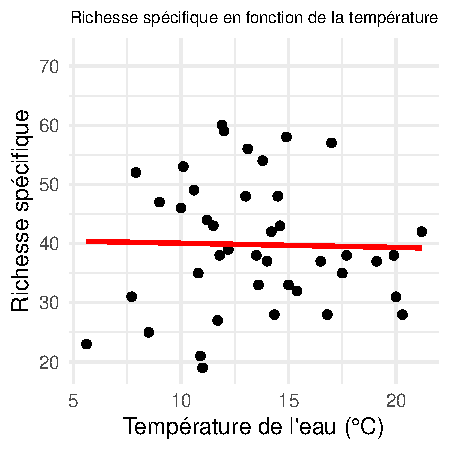
\includegraphics{RMarkdown-article_files/figure-latex/fig_temperature-1} 

}

\caption{Richesse spécifique en fonction de la température de l'eau.}\label{fig:fig_temperature}
\end{figure}

Pour ce qui est des autres régressions, celle de la richesse spécifique
en fonction de la rivière (p=0,293) et la vitesse du courant (p=0,532)
ont respectivement des pentes de -0,2350 et 0,4067, mais ces relations
ne sont pas significatives et ne peuvent donc pas être utilisées pour
expliquer la variation spatiale du benthos. La relation entre la
richesse spécifique et la vitesse du courant est illustrée dans le
deuxième graphique (Figure 2), où la vitesse a été séparée en
différentes catégories, afin de mieux illustrer comment elle varie.

\begin{figure}[H]

{\centering 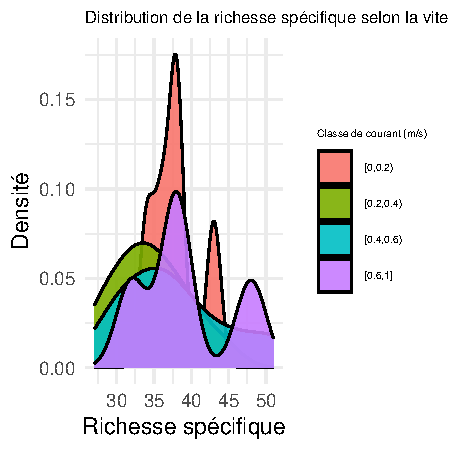
\includegraphics{RMarkdown-article_files/figure-latex/fig_courant-1} 

}

\caption{Richesse spécifique en fonction de la vitesse du courant.}\label{fig:fig_courant}
\end{figure}

Puisque cette relation n'est pas significative, peu de variation est
observée entre les différentes catégories, avec une diversité maximale
lorsqu'il y a entre 0,4 et 0,6m de profondeur. Le graphique (Figure 3)
quant à lui, représente comment la diversité spécifique est distribuée
selon différentes classes de vitesse de courant : plus le pic d'une
courbe est vers la droite et plus il est haut, plus la chance de
retrouver une forte diversité benthique dans cette catégorie de vitesse
est importante.

\begin{figure}

{\centering 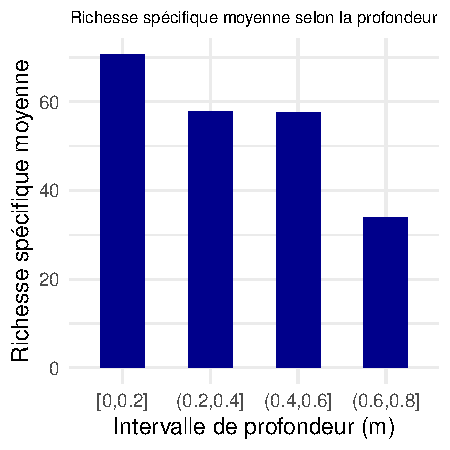
\includegraphics{RMarkdown-article_files/figure-latex/fig_profondeur-1} 

}

\caption{Richesse spécifique en fonction de la profondeur.}\label{fig:fig_profondeur}
\end{figure}

\section{Discussion}\label{discussion}

Selon nos résultats, la profondeur des rivières n'est pas un élément qui
permet d'expliquer la différence dans la distribution spatiale du
benthos, car la corrélation entre les deux variables n'est pas
significative. Ce résultat nous étonne, car plusieurs études, dont une
réalisée au Québec, semblent avoir trouvé un lien entre la profondeur et
la différence en richesse spécifique (1, 3). La profondeur étant liée à
d'autres paramètres comme la luminosité, la température et la
disponibilité en oxygène, un de ces facteurs pourrait peut-être mieux
expliquer la distribution spatiale du benthos. Tel que mentionné dans
les résultats, la vitesse du courant n'est pas significative non plus.
Encore une fois, cela est contraire à ce que l'on s'attendait, puisque
Barmuta et al.@barmuta\_interaction\_1990 et Brysiewicz et al. (1) ont
trouvé une relation significative entre ces variables. Ensuite, tel que
nous l'avions prédit, la température de l'eau a un impact sur la
richesse spécifique du benthos. Cependant, alors que dans les recherches
précédentes la température était un facteur important expliquant
l'évolution spatiale de la diversité benthique, selon notre analyse,
elle n'explique qu'une très petite partie de cette dernière. Hawkins et
al. (4) et Bonacina et al. (5) suggèrent que certains taxons ne peuvent
tolérer des températures trop extrêmes : une régression linéaire simple
ne représente peut-être pas la relation entre la température de l'eau et
la richesse spécifique de la bonne manière, ce qui pourrait expliquer
pourquoi elle explique peu la dispersion spatiale. Ainsi, dans une
prochaine analyse, il serait pertinent de tenter d'expliquer la relation
entre ces deux variables à l'aide d'une autre formule, par exemple la
formule quadratique, afin de prendre en compte la possibilité que l'eau
diminue la diversité benthique lorsqu'elle est trop froide et trop
chaude. De manière semblable, les résultats non-significatifs sont
peut-être expliqués par le fait que la distribution spatiale du benthos
a été étudiée en un seul bloc. Il est possible que certains taxons
soient plus affectés par un paramètre que d'autres, ou qu'ils soient
affectés de manière contraire, ce qui aurait pu nuire à établir une
corrélation significative entre la vitesse du courant ou la profondeur
de la rivière et la richesse spécifique. Finalement, il pourrait être
intéressant faire des analyses multivariées afin de tenter d'avoir des
résultats plus significatifs. Soit en prenant en compte plusieurs des
variables étudiées dans cette présente analyse, soit en prenant en
compte d'autres facteurs qui n'étaient pas présents dans les données
récoltées, tel que le niveau d'oxygénation de l'eau ou sa concentration
en nitrogène, qui sont important pour expliquer la diversité du benthos
(1).

\section*{Réferences}\label{references}
\addcontentsline{toc}{section}{Réferences}

\showmatmethods
\showacknow
\pnasbreak

\phantomsection\label{refs}
\begin{CSLReferences}{0}{1}
\bibitem[\citeproctext]{ref-brysiewicz_characterisation_2022}
\CSLLeftMargin{1. }%
\CSLRightInline{Brysiewicz A, Czerniejewski P, Dąbrowski J, Formicki K
(2022) \href{https://doi.org/10.3390/ani12050606}{Characterisation of
{Benthic} {Macroinvertebrate} {Communities} in {Small} {Watercourses} of
the {European} {Central} {Plains} {Ecoregion} and the {Effect} of
{Different} {Environmental} {Factors}}. \emph{Animals} 12(5):606.}

\bibitem[\citeproctext]{ref-melccfp_macroinvertebres_nodate}
\CSLLeftMargin{2. }%
\CSLRightInline{MELCCFP Macroinvertébrés benthiques. Available at:
\url{https://www.environnement.gouv.qc.ca/eau/eco_aqua/macroinvertebre/benthos/index.htm}
{[}Accessed April 22, 2025{]}.}

\bibitem[\citeproctext]{ref-tall_effects_2016}
\CSLLeftMargin{3. }%
\CSLRightInline{Tall L, Armellin A, Pinel-Alloul B, Méthot G, Hudon C
(2016) \href{https://doi.org/10.1007/s10750-015-2531-7}{Effects of
hydrological regime, landscape features, and environment on
macroinvertebrates in {St}. {Lawrence} {River} wetlands}.
\emph{Hydrobiologia} 778(1):221--241.}

\bibitem[\citeproctext]{ref-hawkins_channel_1997}
\CSLLeftMargin{4. }%
\CSLRightInline{Hawkins CP, Hogue JN, Decker LM, Feminella JW (1997)
\href{https://doi.org/10.2307/1468167}{Channel {Morphology}, {Water}
{Temperature}, and {Assemblage} {Structure} of {Stream} {Insects}}.
\emph{Journal of the North American Benthological Society}
16(4):728--749.}

\bibitem[\citeproctext]{ref-bonacina_effects_2023}
\CSLLeftMargin{5. }%
\CSLRightInline{Bonacina L, Fasano F, Mezzanotte V, Fornaroli R (2023)
\href{https://doi.org/10.1111/brv.12903}{Effects of water temperature on
freshwater macroinvertebrates: A systematic review}. \emph{Biological
Reviews} 98(1):191--221.}

\end{CSLReferences}



% Bibliography
% \bibliography{pnas-sample}

\end{document}
